\documentclass[a4paper]{article}
%\usepackage[margin=2cm]{geometry}

\usepackage{amsmath}
\usepackage{amssymb}
\usepackage{amsfonts}
\usepackage{mathtools}
\usepackage[catalan]{babel} % Language 
\usepackage{fontspec}
\usepackage{graphicx}
\usepackage[makeroom]{cancel}
\usepackage{float}
\usepackage{enumerate}
\usepackage{pgfplots}
\usepackage[hidelinks]{hyperref}

\pgfplotsset{compat=1.13}

\setlength{\parindent}{0pt}
\setlength{\parskip}{0.2cm}

\title{Tema 5: Classificadors generatius}
\author{Joan Marcè Igual}

\begin{document}
	
\maketitle

\section{Introducció}

Un \textbf{classificador} és una funció:
$$
y:\mathbb{R}^d \rightarrow \{ 1,2,...,K \}
$$
$$
K = 2 \rightarrow \text{classificació binària}
$$

Ens interessarà molt trobar mètodes que ofereixin probabilitats. Per exemple:
\begin{align*}
	K = 3 \qquad &x \rightarrow y(x) = "2" \quad (0\ 1\ 0) \quad \text{\textbf{HARD}}\\
	& x \rightarrow y(x) = (0.2, 0.5, 0.3) \quad \text{\textbf{SOFT}}
\end{align*}

Un classificador parteix $\mathbb{R}^d$ en $K$ subconjunts. 

\textbf{Regions de decisió:}

\begin{figure}[H]
	\centering
	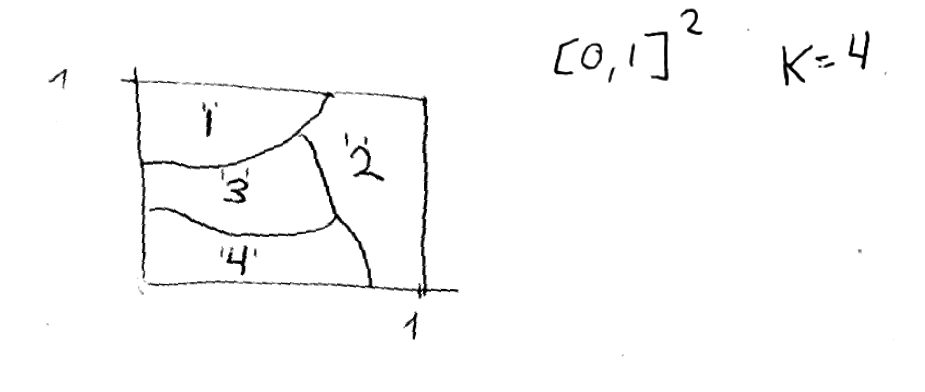
\includegraphics[width=0.5\textwidth]{images/tema_5-1}
\end{figure}

Les regions de decisió estan generades per les zones que delimiten cada classe. Hi ha unes fronteres on les regions canvien. Les separacions es diuen \emph{fronteres de decisió}.

Un classificador és \textbf{lineal} quan només genera fronteres de decisió (entre cada parell de classes) lineals. Per exemple:

\begin{figure}[H]
	\centering
	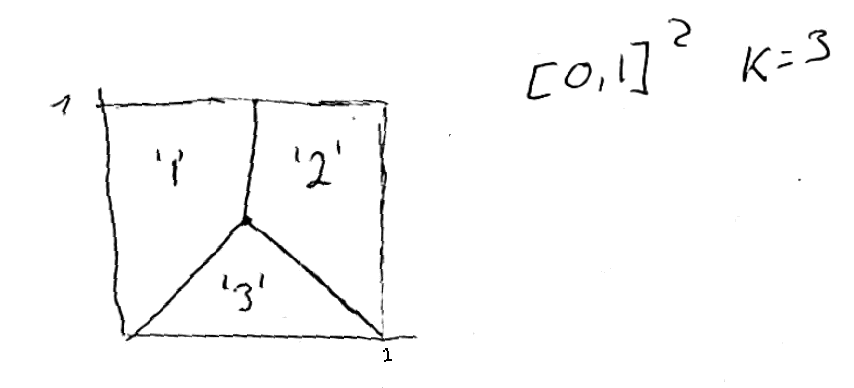
\includegraphics[width=0.5\textwidth]{images/tema_5-2}
\end{figure}

\subsection{La formula de'n Bayes}

Suposem que tenim dues variables aleatòries $A$, $B$, que prenen valors en:

$$
\{ a_1, ..., a_n \}\quad \{ b_1, ..., b_n \}
$$
$$
\begin{cases}
p(a_k) = \sum_{j=1}^n P(a_k, b_j) = \sum_{j=1}^n P(a_k | b_j) P(b_j) \\
P(a_k, b_j) = P(b_j, a_k)
\end{cases}
$$
$$
P(a_k | b_j) P(b_j) = P(b_j | a_k) P(a_k) \implies
\boxed{P(b_j | a_k) = \frac{P(a_k | b_j) P(b_j)}{\sum_{q=1}^n P(a_k | b_q) P(b_q)}}
$$
$$
\sum_{j=1}^m P(b_j | a_k) = 1,\ \forall k 
$$

\textbf{Exemple:} Tenim dues urnes amb pomes ($P$) i taronges ($T$). La probabilitat d'agafar la urna 1 és $\frac{2}{3}$ i la d'agafar la urna 2 és de $\frac{1}{3}$. S'agafa d'una urna a l'atzar un a taronja, quina és la probabilitat que la taronja provingui de la urna 1?

$$
P(U_1|T) =  \frac{P(T|U_1) P(U_1)}{\underbrace{P(T|U_1)P(U_1) + P(T|U_2)P(U_2)}_{P(T)}} =
\frac{\frac{2}{7} · \frac{2}{3}}{\frac{2}{7}·\frac{2}{3} + \frac{7}{9}·\frac{1}{3}} =
\frac{36}{85} < \frac{1}{2}
$$

\begin{figure}[H]
	\centering
	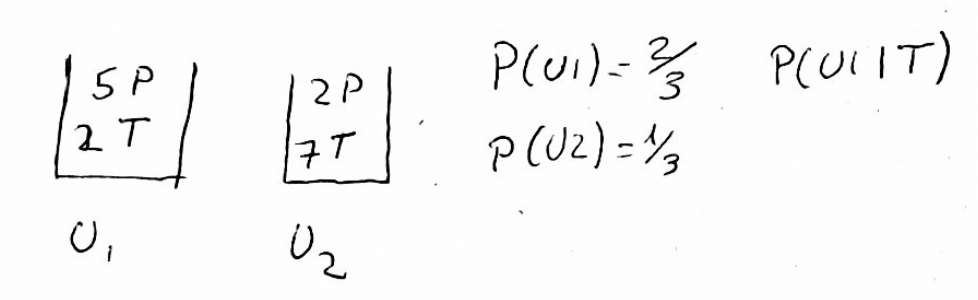
\includegraphics[width=0.7\textwidth]{images/tema_5-3}
\end{figure}

\textbf{Exemple introductori:} Imaginem que tenim un amic ornitòleg que pren mesures de dos tipus d'aus \emph{àligues} i \emph{falcons} i pren mesures de la envergadura (en cm). El nostre amic vol decidir si a partir de la envergadura una au és una àliga o un falcó. 

\begin{figure}[H]
	\centering
	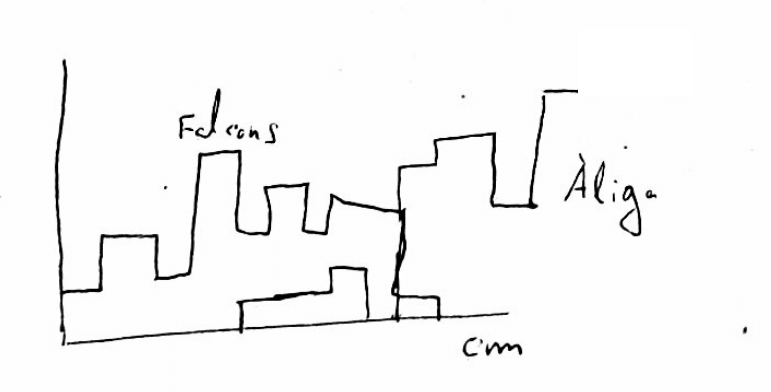
\includegraphics[width=0.7\textwidth]{images/tema_5-4}
\end{figure}

Es tracta de donar una resposta que sigui la òptima. 
$$
N \text{ dades: }
\begin{rcases*}
N_1 \text{ falcons} \\
N_2 \text{ àligues}
\end{rcases*}
\begin{aligned}
C_1 \text{ (falcons)} \\
C_2 \text{ (àligues)}
\end{aligned}
$$

La mida de cada au no és estàndard sinó que varia en funció de l'entorn de manera aleatòria. 

$$
R_1: \text{ la classe de } x = 
\begin{cases}
C_1 \text{ si } \frac{N_1}{N} > \frac{N_2}{N} \\
C_2 \text{ si } \frac{N_2}{N} < \frac{N_1}{N}
\end{cases}
$$ 
Aquesta regla té força errors perquè és constant i no té en compte l'envergadura que hem estat mesurant.

$$
P_{R_1} (error) = \min\left(\frac{N_1}{N}, \frac{N_2}{N}\right) = \frac{1}{N} \min(N_1, N_2)
$$
$$
P_{R_2} (error) = \min(P(C_1), P(C_2))
$$
\begin{align*}
	& P(C_1 | X) = \frac{P(X|C_1)P(C_1)}{P(X|C_1)P(C_1) + P(X|C_2)P(C_2)} \\
	& P(C_2|X) = 1 - P(C_1|X)
\end{align*}

$$
R_{Bayes}: \text{ la classe de } X =
\begin{cases}
C_1 \text{ si } P(C_1|X) > P(C_2|X) \\
C_2 \text{ si } P(C_1|X) < P(C_2|X) \\
\end{cases}
$$
\begin{align*}
&P_{R_{Bays}} (error|X) = min\{P(C_1|X), P(C_2|X)\} \\
&P(error_{total}) = \mathbb{E}(P_{Bayes} (error|X)) = 
\int_{\mathbb{R}} P_{R_{Bays}} (error|X)P(X)dX =
\end{align*}
$$
\int_{\mathbb{R}} \min\{P(C_1|X),P(C_2|X)\}P(X)dX =
$$
$$
\int_{S} \min\left\{\frac{P(X|C_1)P(C_1)}{\cancel{P(X)}}, \frac{P(X|C_2)P(C_2)}{\cancel{P(X)}}\right\}\cancel{P(X)} dX \quad S = \{X|P(X) > 0\} =
$$
$$
\int_S \min\{ P(X|C_1)P(C_1), P(X|C_2)P(C_2) \} dX \le
$$
$$
\min\left\{ \int_S P(X|C_1)P(C_1) dX,\ \int_S P(X|C_2)P(C_2)dX \right\} =
$$
$$
\min\left\{ P(C_1)\int_S P(X|C_1)dX,\ P(C_2)\int_S P(X|C_2)dX \right\} =
$$
$$
\min \{ P(C_1), P(C_2) \} = P_{R_2} (error)
$$

$$
\int_S \min(f_1(x), f_2(x)) dx \le \min\left( \int_S f_1(x) dx,\ \int_S f_2(x) dx \right)
$$

\textbf{Teorema:} La $R_{Bays}$ és la millor regla de decisió (classificació) d'entre les que fan servir $P(C_1|X), P(C_2|X)$.

\section{Classificadors generatius}

$$
P(C_1|X) = \frac{P(X|C_1)P(C_1)}{P(X|C_1)P(C_1) + P(X|C_2)P(C_2)} = 
\frac{1}{1 + \frac{P(X|C_2)P(C_2)}{P(X|C_1)P(C_1)}} =
$$
$$
\text{definim } a(x) := \ln \left( \frac{P(X|C_1)P(C_1)}{P(X|C_2)P(C_2)} \right)
$$
$$
P(C_1|X) = \frac{1}{1 + \exp(-a(x))} = 
$$
$$
\text{definim } g(z) := \frac{1}{1 + e^{-z}} \implies P(C_1|X) = g(a(x))
$$


\subsection{Funció logística}

\begin{figure}[H]
	\centering
	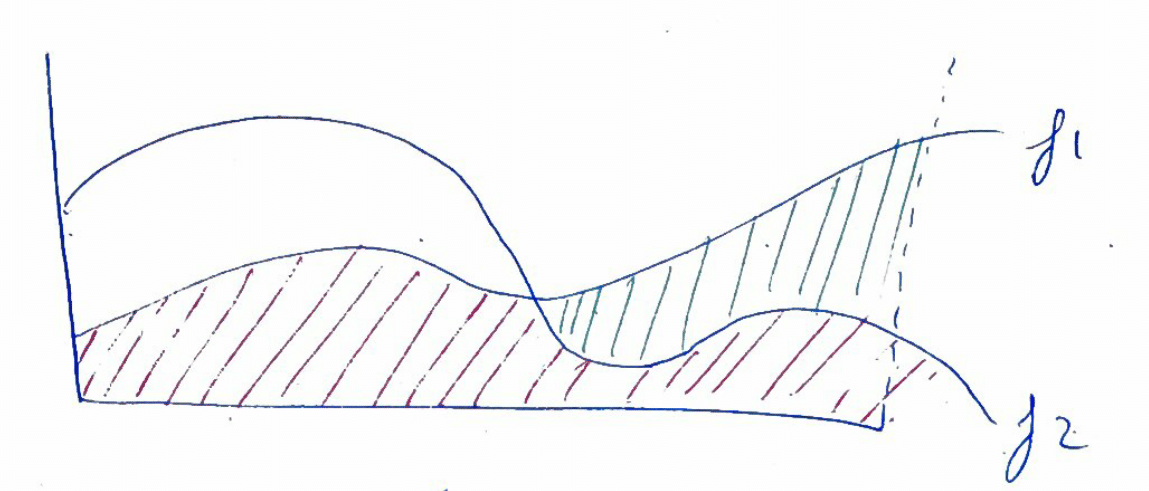
\includegraphics[width=0.8\textwidth]{images/tema_5-5}
\end{figure}

$$
g:\mathbb{R} \rightarrow (0,1)
$$
La funció logística envia tots els valors de $\mathbb{R}$ a un valor comprès entre 0 i 1. Veure \autoref{fig:logistic}

\begin{figure}[H]
	\centering
	\begin{tikzpicture}
	\begin{axis}[
	xmin=-7,xmax=7,ymin=0,ymax=1,
	domain=-10:10
	]
	\addplot+[mark=none] {1/(1 + exp(-x))};
	\end{axis}
	\end{tikzpicture}
	\caption{Gràfic funció logística}
	\label{fig:logistic}
\end{figure}

\begin{itemize}
	\item $ \lim\limits_{z \to +\infty} g(z) = 1 $
	\item $ \lim\limits_{z \to -\infty} g(z) = 0 $
	\item $ g(-z) = 1 - g(z) $
	\item $ g(z) = g(z)[1 - g(z)] $
\end{itemize}

\subsection{Cas de K classes}
$$
1 \le k \le K \qquad P(C_k | X) = \frac{P(X|C_k)P(C_k)}{\sum_{j=1}^K P(X|C_j)P(C_j)} =
$$
$$
\text{definim } a_k(x) = \ln\{P(X|C_k)P(C_k)\}
$$
$$
P(C_k|X) = \frac{\exp(a_k(x))}{\sum_{j=1}^K \exp(a_j(x))} = G_k (a_1(x), a_2(x),...,a_K(x))
$$
$$
G_k(z_1,..,z_K) = \frac{\exp(z_k)}{\sum_{j=1}^N \exp(z_j)} \longrightarrow \text{ softmax}
$$

\section{Aplicació a distribucions Gaussianes}
$$
P(X|C_k) ? \qquad x \in \mathbb{R}^d
$$

Ara suposarem que les dades d'una classe venen d'una Gaussiana multivariable.
$$
P(X|C_k) = N(x, \mu_k, \Sigma_k)
$$

Cas $K=2$
$$
a(x) = \ln \left( \frac{P(X|C_1)P(C_1)}{P(X|C_2)P(C_2)} \right) =
$$
$$
\ln \left( \frac{|\Sigma_1|^{-\frac{1}{2}} 
	\exp\{ -\frac{1}{2}(x - \mu_1)^T \Sigma_1^{-1}(x - \mu_1)^T \} }
	{|\Sigma_2|^{-\frac{1}{2}} 
	\exp\{ -\frac{1}{2}(x - \mu_2)^T \Sigma_2^{-1}(x - \mu_2)^T \}} ·
\frac{P(C_1)}{P(C_2)}\right) =
$$
$$
\frac{1}{2}(x - \mu_2)^T \Sigma_2^{-1} (x - \mu_2) - \frac{1}{2}(x - \mu_1)^T 
\Sigma_1^{-1}(x - \mu_1) + \frac{1}{2}\ln|\Sigma_2| - \frac{1}{2}\ln|\Sigma_1| + 
\ln \frac{P(C_1)}{P(C_2)}
$$

Si $\Sigma_1 = \Sigma_2 = ... = \Sigma_K = \Sigma$ llavors $a_k(x)$ és un \textbf{classificador lineal}.
$$
a_k(x) = w^T x + w_0
$$
\begin{align*}
	& w := \Sigma^{-1}(\mu_1 - \mu_2) \\
	& w_0 := \frac{1}{2} \mu_2^T \Sigma^{-1}\mu_2 - \frac{1}{2}\mu_1^T \Sigma^{-1}\mu_1
	+ \ln \frac{P(C_1)}{P(C_2)}
\end{align*}
$$
P(C_1|X) = g(a(x)) = g(w^Tx + w_0)
$$

\subsection{Estimació dels paràmetres}

\begin{align*}
&	P(C_k) \approx \frac{N_k}{N} \\
&	\mu_k \approx \frac{1}{N_k} \sum_{x_n \in C_k} x_n \\
&	\Sigma_k = \frac{1}{N_k - 1} \sum_{x_n \in C_k} (x_n - \hat{\mu}_k)(x_n - \hat{\mu}_k)^T \\
&	\Sigma_{pooled} = \frac{1}{N - K} \sum_{k=1}^K (N_k - 1) \hat{\Sigma_k}
\end{align*}

\section{Naïve Bayes}
$$
P(C_k|X) = \frac{P(X|C_k)P(C_k)}{P(X)}
$$


$$
P(C_k|X) = \frac{P(x|C_k)P(C_k)}{P(X)} \quad k=1,...,k=K
$$
$$
P(X|C_k) = P(X_1=x_1, X_2=x_2, ..., X_d = x_d|C_k)
$$
$$
x = 
\begin{pmatrix}
x_1 \\ \vdots \\ x_d
\end{pmatrix}, \quad
x \in \mathbb{R}
$$
$$
P(X|C_k) = P(X_1=x_1|C_k)\prod_{j=2}^d P(X_j=x_j|X_1=x_1,X_2=x_2,...,X_{j-1}=x_{j-1}|C_k)
$$
$$
d=3 \rightarrow P(X_1,X_2,X_3) = P(X_3|X_1,X_2)P(X_2|X_1)P(X_1)
$$

$$
P(X|C_k) \underbrace{=}_{\text{naïve}} P(X_1=x_1|C_k) 
\prod_{j=2}^d P(X_j=x_j|C_k) = \prod_{j=1}^d P(X_j=x_j|C_k)
$$
$$
\implies a_k(x) = \ln(P(X|C_k)P(C_k)) = 
\ln\left(P(C_k)\prod_{j=1}^d P(X_j=x_j|C_k)\right) =
$$
$$
= ln P(C_k) + \sum_{j=1}^d \ln P(X_j=x_j|C_k)
$$

\begin{figure}[H]
	\centering
	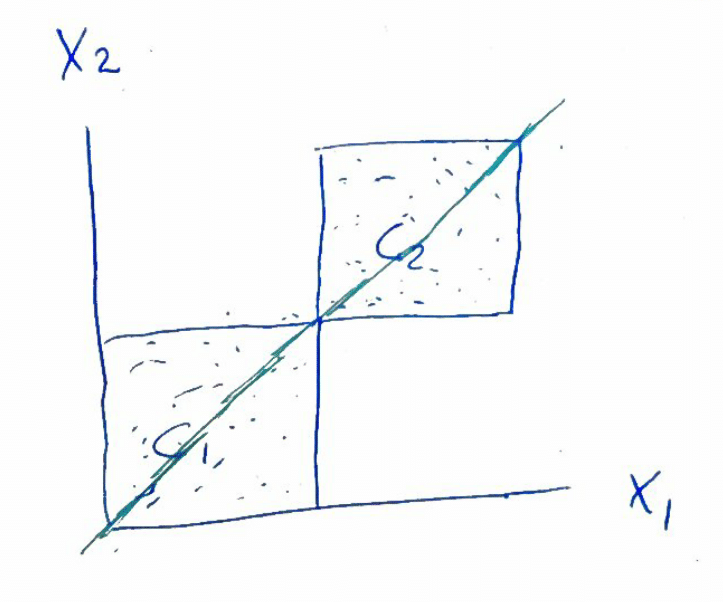
\includegraphics[width=0.7\textwidth]{images/tema_5-6}
\end{figure}

$X_1$ i $X_2$ semblen dependents a primera vista però si només ens centrem en un dels dos conjunts llavors deixen de ser-ho.



\end{document}